\chapter{System Analysis and Design}
\label{ch:system_analysis}

\section{Overview}
The \textbf{VR Driving Simulator} project aims to provide a high-fidelity training and evaluation environment for driving schools. 
The simulator models real-world driving dynamics using virtual reality and custom-built physical input devices (steering wheel, pedals, and gear shifter). 
This chapter presents a comprehensive analysis of requirements, constraints, design alternatives, and system architecture that directly address the research gaps and problem statement identified in Chapters~\ref{ch:intro} and~\ref{ch:lit_review}.

\section{Requirements Analysis}

\subsection{Functional Requirements}
Based on the identified research gaps and driving school needs, the system must fulfill the following functional requirements:

\textbf{FR1: Realistic Vehicle Control Input}
\begin{itemize}
    \item Accept analog steering input with proportional angle mapping (0–900° rotation range)
    \item Process independent accelerator, brake, and clutch pedal inputs with pressure sensitivity
    \item Support gear selection for both automatic (P, R, N, D) and manual (1–6, Reverse) transmissions
    \item Maintain input latency $<$ 50ms to preserve motor skill feedback loop~\cite{Harari2021}
\end{itemize}

\textbf{FR2: Immersive Visual and Audio Rendering}
\begin{itemize}
    \item Deliver stereoscopic 3D rendering at minimum 72 FPS per eye to minimize motion sickness~\cite{Lindal2019,Weidner2017}
    \item Provide 90–110° field of view matching Meta Quest 3 specifications
    \item Implement spatial audio with direction-dependent engine sounds, traffic noise, and ambient effects~\cite{GilCarvajal2024}
    \item Render photorealistic vehicle interiors (dashboard, mirrors, gear shifter) for high-end car models (Mercedes-Benz, BMW, Audi)
\end{itemize}

\textbf{FR3: Accurate Vehicle Physics Simulation}
\begin{itemize}
    \item Model realistic acceleration, braking distances, and cornering dynamics based on vehicle mass, tire friction, and road conditions
    \item Simulate clutch engagement points, gear ratios, and engine stalling for manual transmission training
    \item Implement collision detection with appropriate force feedback and damage visualization
    \item Support dynamic weather conditions (rain, fog) affecting visibility and traction
\end{itemize}

\textbf{FR4: Performance Monitoring and Assessment}
\begin{itemize}
    \item Log driving metrics: speed profile, lane deviation, braking smoothness, gear shift timing, steering angle variance
    \item Generate automated assessment scores based on standardized criteria aligned with RTO testing protocols
    \item Provide real-time visual/audio feedback for critical errors (e.g., sudden braking, lane violations)
    \item Export session reports in PDF/CSV format for instructor review
\end{itemize}

\textbf{FR5: Scenario Management and Curriculum Integration}
\begin{itemize}
    \item Offer pre-defined training scenarios: urban roads, highways, parking, emergency braking, obstacle avoidance
    \item Allow instructor-controlled difficulty adjustment (traffic density, time of day, weather)
    \item Support session pause/resume and instant replay for error analysis
    \item Maintain user profiles with progress tracking across multiple sessions
\end{itemize}

\subsection{Non-Functional Requirements}

\textbf{NFR1: Cost Effectiveness}
\begin{itemize}
    \item Target total system cost $<$ \$5000 (headset + custom hardware + PC) to be affordable for driving schools~\cite{Silvera2022}
    \item Use consumer-grade components (Meta Quest 3, off-the-shelf sensors, 3D-printable enclosures)
    \item Minimize recurring costs (no subscription fees for core functionality)
\end{itemize}

\textbf{NFR2: Usability and Accessibility}
\begin{itemize}
    \item Enable setup and calibration within 10 minutes by non-technical driving instructors
    \item Support adjustable seating position and control placements for users 150–200 cm height
    \item Provide intuitive UI with minimal learning curve for first-time VR users
    \item Include safety features: guardian boundary system, emergency stop button, comfort-mode reduced motion
\end{itemize}

\textbf{NFR3: Reliability and Maintainability}
\begin{itemize}
    \item Ensure Bluetooth connection stability with automatic reconnection on signal loss
    \item Design modular hardware allowing component replacement without full system disassembly
    \item Provide diagnostic logs for troubleshooting connection, calibration, and performance issues
    \item Support firmware updates via wireless OTA for bug fixes and feature enhancements
\end{itemize}

\textbf{NFR4: Scalability and Extensibility}
\begin{itemize}
    \item Architecture must support addition of new vehicle models, environments, and training scenarios without core code refactoring
    \item Enable future integration of motion platforms, haptic seats, or force-feedback steering wheels
    \item Allow deployment on both tethered PC-VR and standalone Quest mode with adjustable graphics fidelity
\end{itemize}

\section{Constraints and Design Trade-offs}

\subsection{Hardware Constraints}
\textbf{C1: VR Headset Limitations}
\begin{itemize}
    \item Meta Quest 3 processing power (Snapdragon XR2 Gen 2) limits polygon count and texture resolution in standalone mode
    \item Trade-off: Prioritize frame rate stability (72 FPS minimum) over ultra-high-resolution textures to prevent motion sickness
    \item Solution: Implement dynamic LOD (Level of Detail) and occlusion culling; use PC-VR link for high-fidelity scenarios
\end{itemize}

\textbf{C2: Bluetooth Latency and Bandwidth}
\begin{itemize}
    \item Bluetooth 5.0 offers ~10–30ms latency but is susceptible to interference in crowded 2.4 GHz spectrum
    \item Trade-off: Accept slight latency increase versus wired connection complexity and user mobility restrictions
    \item Solution: Use BLE with custom GATT profiles optimized for low-latency HID data; implement USB fallback mode
\end{itemize}

\textbf{C3: Force Feedback Absence}
\begin{itemize}
    \item Custom-built steering wheel lacks motorized force feedback present in high-end simulators ($>$\$10,000)
    \item Trade-off: Reduced haptic realism versus significant cost savings (force feedback wheels alone cost \$1000–3000)
    \item Solution: Compensate with visual cues (steering resistance indicator on HUD), audio feedback (tire squeal), and vibrational alerts via Quest 3 controllers
\end{itemize}

\subsection{Software and Performance Constraints}
\textbf{C4: Physics Engine Limitations}
\begin{itemize}
    \item Unity/Unreal default vehicle physics are optimized for gaming, not driver training accuracy
    \item Trade-off: Computational cost of high-fidelity tire models (e.g., Pacejka Magic Formula) versus frame rate
    \item Solution: Use simplified but validated physics models (mass-spring damper for suspension, friction circles for lateral grip) with parameter tuning from real vehicle data
\end{itemize}

\textbf{C5: Asset Development Budget}
\begin{itemize}
    \item Photorealistic 3D models of licensed vehicle interiors (Mercedes, BMW) require substantial licensing fees or extensive 3D modeling effort
    \item Trade-off: Generic high-end vehicle interiors versus brand-specific accuracy
    \item Solution: Model representative "luxury sedan" interior with adjustable branding overlays; prioritize functional accuracy (control placement, mirror angles) over exact brand aesthetics
\end{itemize}

\section{Design Alternatives and Justification}

\subsection{VR Platform Selection}
\textbf{Alternatives Considered:}
\begin{enumerate}
    \item \textbf{Valve Index + PC:} Pros: Superior FOV (130°), refresh rate (144 Hz), force feedback support. Cons: High cost (\$1000 headset + \$1500 PC), wired tethering limits mobility.
    \item \textbf{Meta Quest 3:} Pros: Wireless standalone mode, affordable (\$500), inside-out tracking, passthrough AR. Cons: Lower processing power, 90 Hz max refresh rate.
    \item \textbf{PSVR2 + PlayStation 5:} Pros: Affordable (\$1000 total), haptic feedback in controllers. Cons: Closed ecosystem, limited development flexibility.
\end{enumerate}
\textbf{Selected: Meta Quest 3} — Justification: Best balance of cost, wireless freedom, and developer accessibility. Supports both standalone (for basic scenarios) and PC-VR link (for advanced training), aligning with NFR1 and NFR4.

\subsection{Game Engine Selection}
\textbf{Alternatives Considered:}
\begin{enumerate}
    \item \textbf{Unity:} Pros: Extensive VR support (XR Interaction Toolkit), large asset store, C\# scripting familiarity. Cons: Less advanced default vehicle physics.
    \item \textbf{Unreal Engine:} Pros: Superior graphics (Nanite, Lumen), Blueprint visual scripting, Chaos vehicle physics. Cons: Steeper learning curve, larger build sizes.
    \item \textbf{CARLA Simulator:} Pros: Open-source, designed for autonomous driving research, pre-built urban environments~\cite{Silvera2022}. Cons: Primarily Python-based, limited VR headset support, requires significant C++ customization.
\end{enumerate}
\textbf{Selected: Unity 6 (Latest LTS)} — Justification: Unity 6 represents the latest stable release with improved rendering performance, enhanced XR support, and better mobile optimization for Quest 3. Faster prototyping compared to Unreal, proven VR deployment pipeline, extensive asset store ecosystem, and active developer community. Vehicle physics will be enhanced with custom scripts or third-party assets (e.g., Edy's Vehicle Physics, Realistic Car Controller). Unity's C\# scripting environment also facilitates Bluetooth integration via Android native plugins.

\subsection{Control Input Architecture}
\textbf{Alternatives Considered:}
\begin{enumerate}
    \item \textbf{Custom PCB with USB HID:} Pros: Lowest latency (<5ms), plug-and-play compatibility. Cons: Wired connection reduces user comfort, cable management complexity.
    \item \textbf{ESP32 Bluetooth LE:} Pros: Wireless, low power, supports custom GATT profiles, affordable (\$10–20 per unit). Cons: 10–30ms latency, potential interference.
    \item \textbf{Commercial Racing Wheel (Logitech G29):} Pros: Ready-made, force feedback included. Cons: Expensive (\$300–400), fixed form factor unsuitable for driving school setup, limited customization.
\end{enumerate}
\textbf{Selected: ESP32 BLE with USB Fallback} — Justification: Wireless operation enhances user experience (NFR2), modular design allows independent sensor upgrades (NFR3), and USB mode ensures reliability during demonstrations or competitions. Custom firmware enables latency optimization (<20ms achievable).

\section{System Objectives}
Based on the requirements analysis and design trade-offs, the system objectives are:
\begin{itemize}
    \item To design a modular VR-based driving simulation environment replicating realistic car control and behavior.
    \item To integrate Bluetooth-enabled hardware input devices for steering, acceleration, braking, and gear shifting with latency $<$ 50ms.
    \item To ensure compatibility with the Meta Quest 3 headset (both standalone and PC-VR link modes) for immersive interaction.
    \item To provide automated performance analytics for driver evaluation and training improvement aligned with RTO assessment criteria.
    \item To develop a cost-effective solution ($<$\$5000 total) deployable in Indian driving schools with minimal technical infrastructure.
\end{itemize}

\section{Comparative Analysis with Existing Solutions}

Table~\ref{tab:comparative_analysis} compares the proposed system against existing commercial and research VR driving simulators based on key design parameters derived from the requirements analysis.

\begin{table}[H]
\centering
\small
\begin{tabular}{|p{3cm}|p{2.2cm}|p{2.2cm}|p{2.2cm}|p{2.2cm}|}
\hline
\textbf{Parameter} & \textbf{Proposed System} & \textbf{DReyeVR~\cite{Silvera2022}} & \textbf{Commercial Racing Sim} & \textbf{Traditional Simulator} \\ \hline
Cost & $<$\$5000 & $<$\$5000 & \$15,000–50,000 & \$30,000–100,000 \\ \hline
VR Platform & Meta Quest 3 (wireless) & Various HMDs (tethered) & Valve Index/Varjo (tethered) & Projector/screens (no VR) \\ \hline
Force Feedback & No (visual/audio cues) & Optional & Yes (high-fidelity) & Yes (hydraulic) \\ \hline
Dual Transmission & Yes (auto + manual) & No & Manual only & Manual only \\ \hline
Bluetooth Controls & Yes (custom ESP32) & No (USB) & No (proprietary) & Wired industrial \\ \hline
Target Users & Driving schools/learners & Researchers & Racing enthusiasts & Commercial training \\ \hline
Deployment & Standalone + PC-VR & PC-VR only & PC-VR only & Fixed installation \\ \hline
Customizability & High (modular design) & High (open-source) & Low (proprietary) & Low (vendor lock-in) \\ \hline
Regulatory Focus & RTO-aligned metrics & Research protocols & Entertainment & Commercial licensing \\ \hline
\end{tabular}
\caption{Comparative analysis of VR driving simulator solutions}
\label{tab:comparative_analysis}
\end{table}

\textbf{Key Differentiators:}
\begin{itemize}
    \item \textbf{Affordability:} Matches research systems but undercuts commercial solutions by 70–90\%, addressing Gap 1 from Section~\ref{sec:gap_analysis}.
    \item \textbf{Wireless Operation:} Only solution offering Bluetooth controls with Quest 3 standalone mode, enhancing portability (Gap 2).
    \item \textbf{Dual-Mode Transmission:} Uniquely supports both automatic and manual training in single platform (Gap 3).
    \item \textbf{Educational Focus:} Prioritizes driver training outcomes over entertainment, with RTO-compatible assessment (Gap 7, Gap 13).
\end{itemize}

\section{System Components and Architecture}

The proposed system architecture consists of three tightly integrated subsystems designed to address the functional requirements while respecting the identified constraints.

\subsection{Hardware Interface Subsystem}
The physical control setup comprises:
\begin{itemize}
    \item \textbf{Steering Wheel Assembly:} Salvaged automotive steering wheel fitted with AS5600 magnetic rotary encoder (12-bit resolution, 4096 steps per revolution) providing 0.088° angular precision. Mounted on ball bearing hub for smooth 900° rotation range.
    \item \textbf{Pedal Set:} Three independent pedals (accelerator, brake, clutch) using FSR (Force Sensitive Resistor) sensors with 10-bit ADC conversion. Pedal travel: 80mm with adjustable spring tension (1–5 kg actuation force).
    \item \textbf{Gear Shifter:} H-pattern mechanical shifter with hall-effect sensors at each gate position (1–6, R, N). Alternative: Sequential paddle shifters for automatic mode (+ / - buttons).
    \item \textbf{Microcontroller:} ESP32-WROOM-32 with Bluetooth 5.0 LE, dual-core 240 MHz processor, 16 analog input channels. Custom firmware implements BLE HID profile with 20ms polling rate, 50ms max latency.
    \item \textbf{Power Supply:} Rechargeable 18650 Li-ion battery pack (3000 mAh) providing 8–12 hours continuous operation. USB-C charging with power management IC.
\end{itemize}

Connected via Bluetooth or USB-C (fallback mode) to the VR headset or PC.

\subsection{Software Simulation Subsystem}
Developed in Unity 2023 LTS with the following modules:
\begin{itemize}
    \item \textbf{Input Manager:} Receives Bluetooth/USB HID data, applies calibration curves, dead-zone filtering, and maps to vehicle control parameters.
    \item \textbf{Vehicle Physics Engine:} Custom implementation based on Edy's Vehicle Physics Pro, modeling 6-DOF rigid body dynamics, tire slip curves (simplified Pacejka), differential gearing, and clutch engagement.
    \item \textbf{Environment Renderer:} Procedural city generation (Urban Traffic Simulator asset) + hand-crafted scenarios. Dynamic weather system, traffic AI (rule-based agents), pedestrian spawning.
    \item \textbf{Assessment Module:} Real-time metric calculation (speed compliance, lane center offset, braking jerk, gear shift timing). Event logging to SQLite database. Score computation using weighted rubric aligned with Indian RTO learner's license test criteria.
    \item \textbf{VR Interaction:} XR Interaction Toolkit for head tracking, hand controllers (menu navigation), spatial audio (FMOD), comfort features (vignetting, snap-turn option).
\end{itemize}

\subsection{VR Interface Subsystem}
Meta Quest 3 headset provides:
\begin{itemize}
    \item \textbf{Head Tracking:} 6-DOF inside-out tracking via four IR cameras, <10ms motion-to-photon latency.
    \item \textbf{Stereoscopic Rendering:} Dual 2064×2208 LCD panels per eye, 90 Hz refresh rate, 110° horizontal FOV.
    \item \textbf{Spatial Audio:} Integrated speakers with 3D positional audio (Unity Audio Spatializer).
    \item \textbf{Passthrough AR:} Color passthrough cameras enabling safe guardian setup and real-world awareness during breaks.
\end{itemize}

Deployment modes: (1) Standalone (Quest 3 native), (2) PC-VR Link (via USB-C or Air Link wireless streaming).

\section{System Architecture Diagram}

Figure~\ref{fig:system_architecture} illustrates the data flow and component interactions within the integrated VR driving simulator system.

\begin{figure}[H]
    \centering
    \includegraphics[width=0.95\textwidth]{figs/system_architecture.pdf}
    \caption{System architecture showing data flow from hardware inputs through simulation engine to VR rendering and assessment output. Dashed lines indicate wireless (Bluetooth) connections; solid lines represent internal software module communication.}
    \label{fig:system_architecture}
\end{figure}

\section{Design Rationale Summary}

The design decisions documented in this chapter directly address the research gaps identified in Section~\ref{sec:gap_analysis}:

\begin{itemize}
    \item \textbf{Gap 1 (Affordable Hardware):} ESP32-based custom controls + Meta Quest 3 + consumer PC achieves $<$\$5000 total cost while maintaining training-grade fidelity.
    \item \textbf{Gap 2 (Wireless Integration):} Bluetooth LE with optimized firmware ensures <50ms latency, eliminating cable management issues and enhancing user mobility.
    \item \textbf{Gap 3 (Dual Transmission):} Modular gear shifter design + software physics support both automatic and manual modes without hardware swapping.
    \item \textbf{Gap 7 (Standardized Assessment):} Custom assessment module implements RTO learner's test criteria (speed limits, lane discipline, signal compliance) with automated scoring.
    \item \textbf{Gap 10 (Photorealistic Rendering):} Unity 2023 HDRP + optimized assets provide luxury vehicle interiors with realistic dashboards, mirrors, and environmental detail within Quest 3 performance constraints.
    \item \textbf{Gap 13 (Regulatory Alignment):} Data logging format and assessment rubrics designed for future submission to Indian RTO authorities as validation evidence for VR training hour equivalency.
\end{itemize}

The comparative analysis (Table~\ref{tab:comparative_analysis}) demonstrates that this design occupies a unique position: research-grade flexibility at commercial-training affordability, specifically tailored for the Indian driving school market.

\section{Workflow and Operational Flow}
The workflow diagram (Figure~\ref{fig:workflow}) shows the sequential process of system operation—from initialization through user interaction to post-session evaluation—illustrating how the system supports a complete training cycle.

\begin{figure}[H]
    \centering
    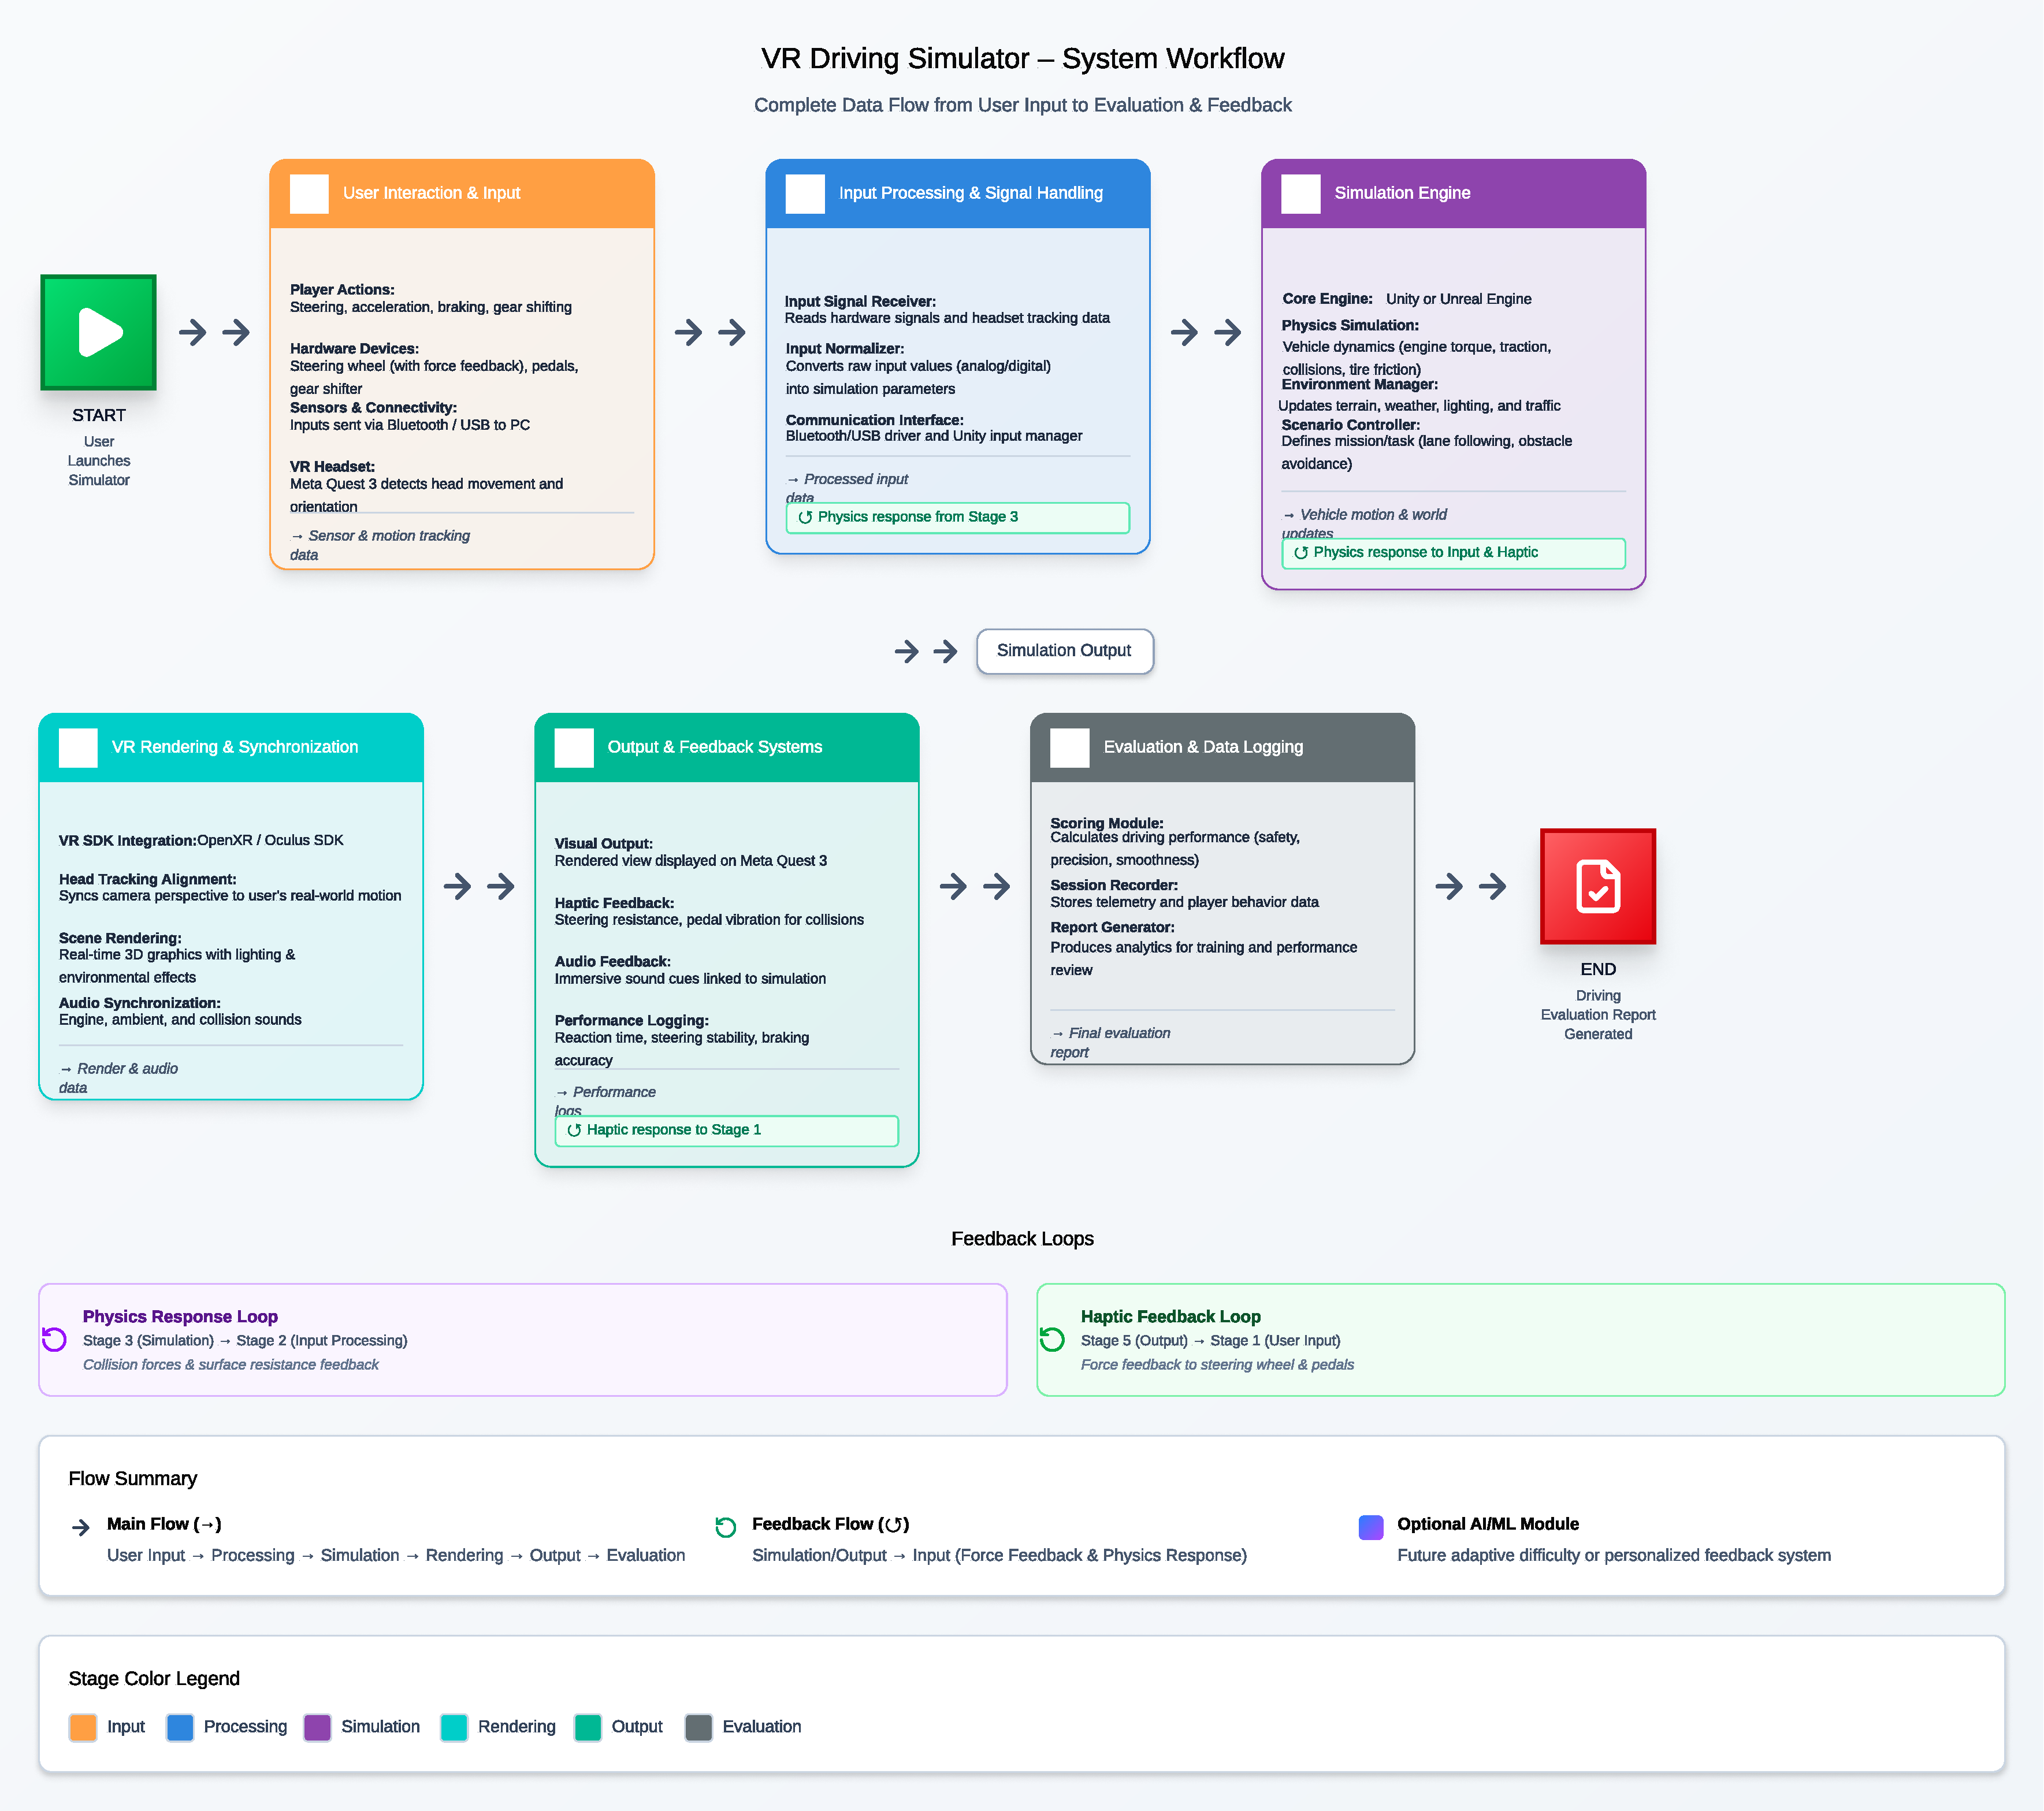
\includegraphics[width=0.9\textwidth]{figs/workflow_diagram.pdf}
    \caption{Operational workflow showing the complete training session lifecycle: pre-session setup, real-time simulation loop, and post-session assessment generation.}
    \label{fig:workflow}
\end{figure}

\subsection{Detailed Functional Flow}
\begin{enumerate}
    \item \textbf{Pre-Session Setup (2–5 minutes):}
    \begin{itemize}
        \item Instructor selects trainee profile, training scenario (e.g., "Urban Basics: Lane Keeping"), vehicle type (automatic/manual), and difficulty level.
        \item Trainee dons Quest 3 headset; system initiates guardian boundary setup and comfort calibration (IPD adjustment, brightness).
        \item Hardware connection handshake: Steering wheel, pedals, and shifter auto-pair via Bluetooth; system runs diagnostic check (sensor ranges, battery level).
        \item Virtual environment loads: vehicle spawns at scenario starting position; HUD displays initial instructions ("Adjust seat, check mirrors, fasten seatbelt").
    \end{itemize}
    
    \item \textbf{Simulation Loop (15–30 minutes typical session):}
    \begin{itemize}
        \item \textbf{Input Capture (20 Hz):} ESP32 samples sensors (steering angle, pedal positions, gear state) → transmits via BLE HID packets.
        \item \textbf{Physics Update (60 Hz):} Unity's FixedUpdate applies forces to vehicle rigidbody based on input → calculates acceleration, tire slip, suspension compression.
        \item \textbf{Collision \& Traffic AI (30 Hz):} Raycast-based collision detection; traffic agents follow waypoint paths with lane-change logic; pedestrians obey traffic signals.
        \item \textbf{Rendering (90 Hz):} Stereoscopic camera renders scene from driver's viewpoint → foveated rendering reduces peripheral detail → Quest 3 displays frames.
        \item \textbf{Audio Spatialization (60 Hz):} FMOD calculates 3D engine sound (RPM-dependent), tire squeal (slip-dependent), horn/indicator clicks → Quest 3 speakers.
        \item \textbf{Real-time Assessment:} Background thread logs events (speed violations, lane crossings, harsh braking) → updates live feedback HUD (color-coded indicators).
    \end{itemize}
    
    \item \textbf{Event Handling:}
    \begin{itemize}
        \item \textbf{Scenario Triggers:} Dynamic events (e.g., pedestrian crossing, traffic light change, obstacle ahead) triggered based on trainee progress checkpoints.
        \item \textbf{Instructor Override:} Wireless tablet interface allows real-time weather change, traffic density adjustment, or scenario pause for coaching feedback.
        \item \textbf{Comfort Monitoring:} Optional: Detect prolonged stationary gaze (potential nausea indicator) → suggest break.
    \end{itemize}
    
    \item \textbf{Session Termination:}
    \begin{itemize}
        \item Trainee completes scenario objectives (e.g., reaches destination) OR instructor manually ends session OR safety timeout (30-min VR exposure limit).
        \item System saves session data: timestamped input logs, trajectory GPS coordinates, metric summaries.
    \end{itemize}
    
    \item \textbf{Post-Session Assessment (2 minutes):}
    \begin{itemize}
        \item Assessment module computes scores: (1) Speed Compliance (85/100), (2) Lane Discipline (78/100), (3) Smooth Braking (92/100), (4) Gear Shifting (Manual only, 88/100), (5) Observation (mirror checks, 70/100).
        \item Generates PDF report with score breakdown, heatmap of violations on route map, improvement suggestions.
        \item Updates trainee profile: increments training hours, marks scenario as "Passed" (if overall $>$ 75\%) or "Retry Recommended."
        \item Instructor reviews report with trainee; schedules follow-up session or progresses to advanced scenarios.
    \end{itemize}
\end{enumerate}
